%%==============================================================
%% Modelo de Dissertação de Mestrado para o mestrado de Ciência da Computação
%% da Universidade Federal de Viçosa 
%% Adaptado por: Marcelo Menezes e Gabriel Franco
%% Ultima versao
%% Arquivo em formato UTF-8
%% Compilar com pdftex
% %Precisa do arquivo abntex2-UFV.sty
%%==============================================================

\documentclass[
	% -- opções da classe memoir --
	12pt,				    % tamanho da fonte
	openright,			    % capítulos começam em pág ímpar (insere página vazia caso preciso)
	oneside,			    % para impressão só no anverso. Oposto a twoside
	a4paper,			    % tamanho do papel.
    % -- opções do pacote abntex2 --
    % chapter=TITLE,         % Títulos em maiúsculas
    sumario=tradicional,    % Sumário padrão memoir (mais bonito "imo")
    % -- opções do pacote babel --
	brazil,				    % idioma adicional para hifenização
	brazil,			    % o último idioma é o principal do documento
	]{abntex2}              % Personaliza a capa. Precisa do arquivo ufv.cls para funcionar.


\usepackage{adjustbox}
% Pacotes fundamentais
\usepackage{abntex2-UFV}        % Personalização para a Universidade Federal de Viçosa
\usepackage{lmodern}			% Usa a fonte Latin Modern			
\usepackage[T1]{fontenc}		% Selecao de codigos de fonte de saída
\usepackage[utf8]{inputenc}		% Codificacao do documento (conversão automática dos acentos)
\usepackage{indentfirst}		% Indenta o primeiro parágrafo de cada seção.
\usepackage{graphicx}			% Inclusão de gráficos
\usepackage[table,xcdraw]{xcolor}
\usepackage{booktabs}           % \toprule, \midrule e \bottomrule para tabelas
% Sistema autor-data com títulos nas referências em negrito
\usepackage[alf,abnt-emphasize=bf]{abntex2cite}	

\usepackage{amsmath}
\usepackage{amssymb}
\usepackage{pdfpages}
%--------------------------------------------------------- MY STUFF
\usepackage{mathtools}
\DeclarePairedDelimiter{\ceil}{\lceil}{\rceil}
\DeclarePairedDelimiter{\floor}{\lfloor}{\rfloor}

\usepackage{listings}
\usepackage{subcaption}

\usepackage{caption}

\usepackage{xurl}

\DisemulatePackage{setspace}
\usepackage{setspace}
\usepackage[linesnumbered,lined,commentsnumbered,ruled,vlined,portuguese]{algorithm2e}
\usepackage{bm}
\usepackage{multirow}
\usepackage{lipsum}
%------------------------------------------------------------------

\SetKwFor{ParaCada}{para cada}{fa\c{c}a}{fim para}
\hyphenation{fe-de-ral}
\hyphenation{scientiae}

% ---
% CONFIGURAÇÕES DE PACOTES
% ---

% Informações de dados para CAPA e FOLHA DE ROSTO
\titulo{\normalsize{\textbf{Título da dissertação}}}
\autor{\normalsize{\textbf{John Doe}}}
\local{\normalsize{\textbf{Viçosa - Minas Gerais}}}
\data{\normalsize{\textbf{2021}}}
\orientador{Nome do Orientador}    % redefinido no abntex2-UFV para aceitar Instituição (default = UFV)
%\coorientador{Nome do Coorientador}
\instituicao{Universidade Federal de Viçosa}
\curso{Pós-graduação em Ciência da Computação}               % pacote abntex2-UFV
\membrobancaA{Membro 1}             % pacote abntex2-UFV default = UFV
\membrobancaB{Membro 2}       % pacote abntex2-UFV default = UFV
\databanca{\today}                           % pacote abntex2-UFV

% O preambulo deve conter o tipo do trabalho, o objetivo,
% o nome da instituição e a área de concentração

\preambulo{Dissertação apresentada à Universidade Federal de Viçosa, como parte das exigências do Programa de Pós-Graduação em Ciência da Computação, para obtenção do título de \textit{Magister Scientiae}.}
%\preambulo{Dissertation submitted to the Computer Science Graduate Program of Universidade Federal de Viçosa in partial fulfillment of the requirements for the degree of \textit{Magister Scientiae}.}
% ---

% ---
% Configurações de aparência do PDF final

% informações para o arquivo pdf de saída
% Interessante alterar a cor dos links para preto(black)
% para imprimir
\makeatletter
\hypersetup{
        % metadados
		pdftitle={\@title},
		pdfauthor={\@author},
    	pdfsubject={\imprimirpreambulo},
	    pdfcreator={LaTeX with abnTeX2},
		colorlinks=true,   % false: links em frame; true: links coloridos
    	linkcolor=black,    % cor dos links no documento
    	citecolor=blue,    % cor dos links para a bibliografia
    	filecolor=magenta, % cor dos links para arquivos
		urlcolor=blue,     % cor dos links para sites
		bookmarksdepth=4   % profundidade do sumário do PDF
}
\makeatother
% ---

\begin{document}
% Retira espaço extra obsoleto entre as frases.
\frenchspacing

% ----------------------------------------------------------
% ELEMENTOS PRÉ-TEXTUAIS
% ----------------------------------------------------------
\pretextual

% Capa
%\imprimircapa

% Folha de rosto
{
    \singlespacing
    \imprimirfolhaderosto
    \clearpage
    \pagenumbering{arabic}
}
% ---

% Ficha catalográfica
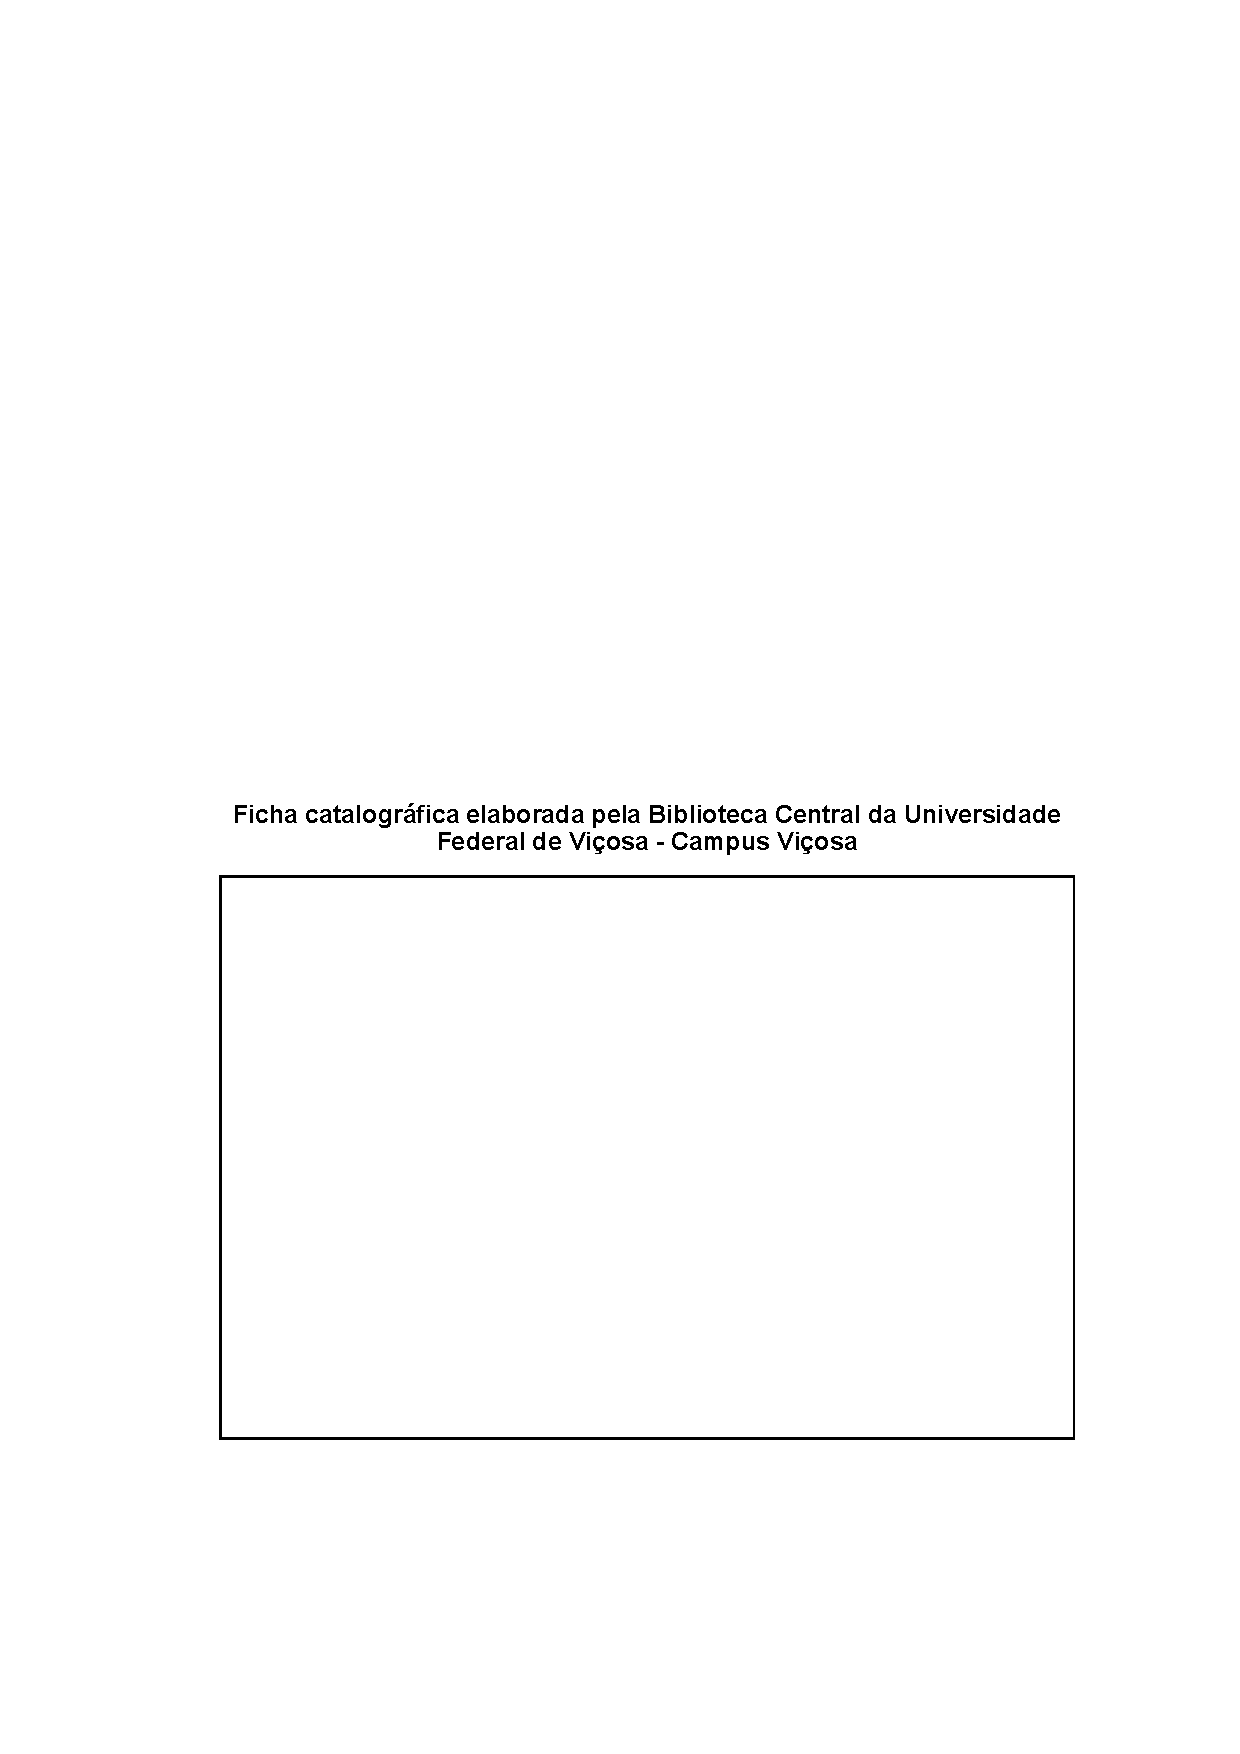
\includepdf[pages=-]{pdfs/ficha-catalografica-branca.pdf}

% Folha de aprovação
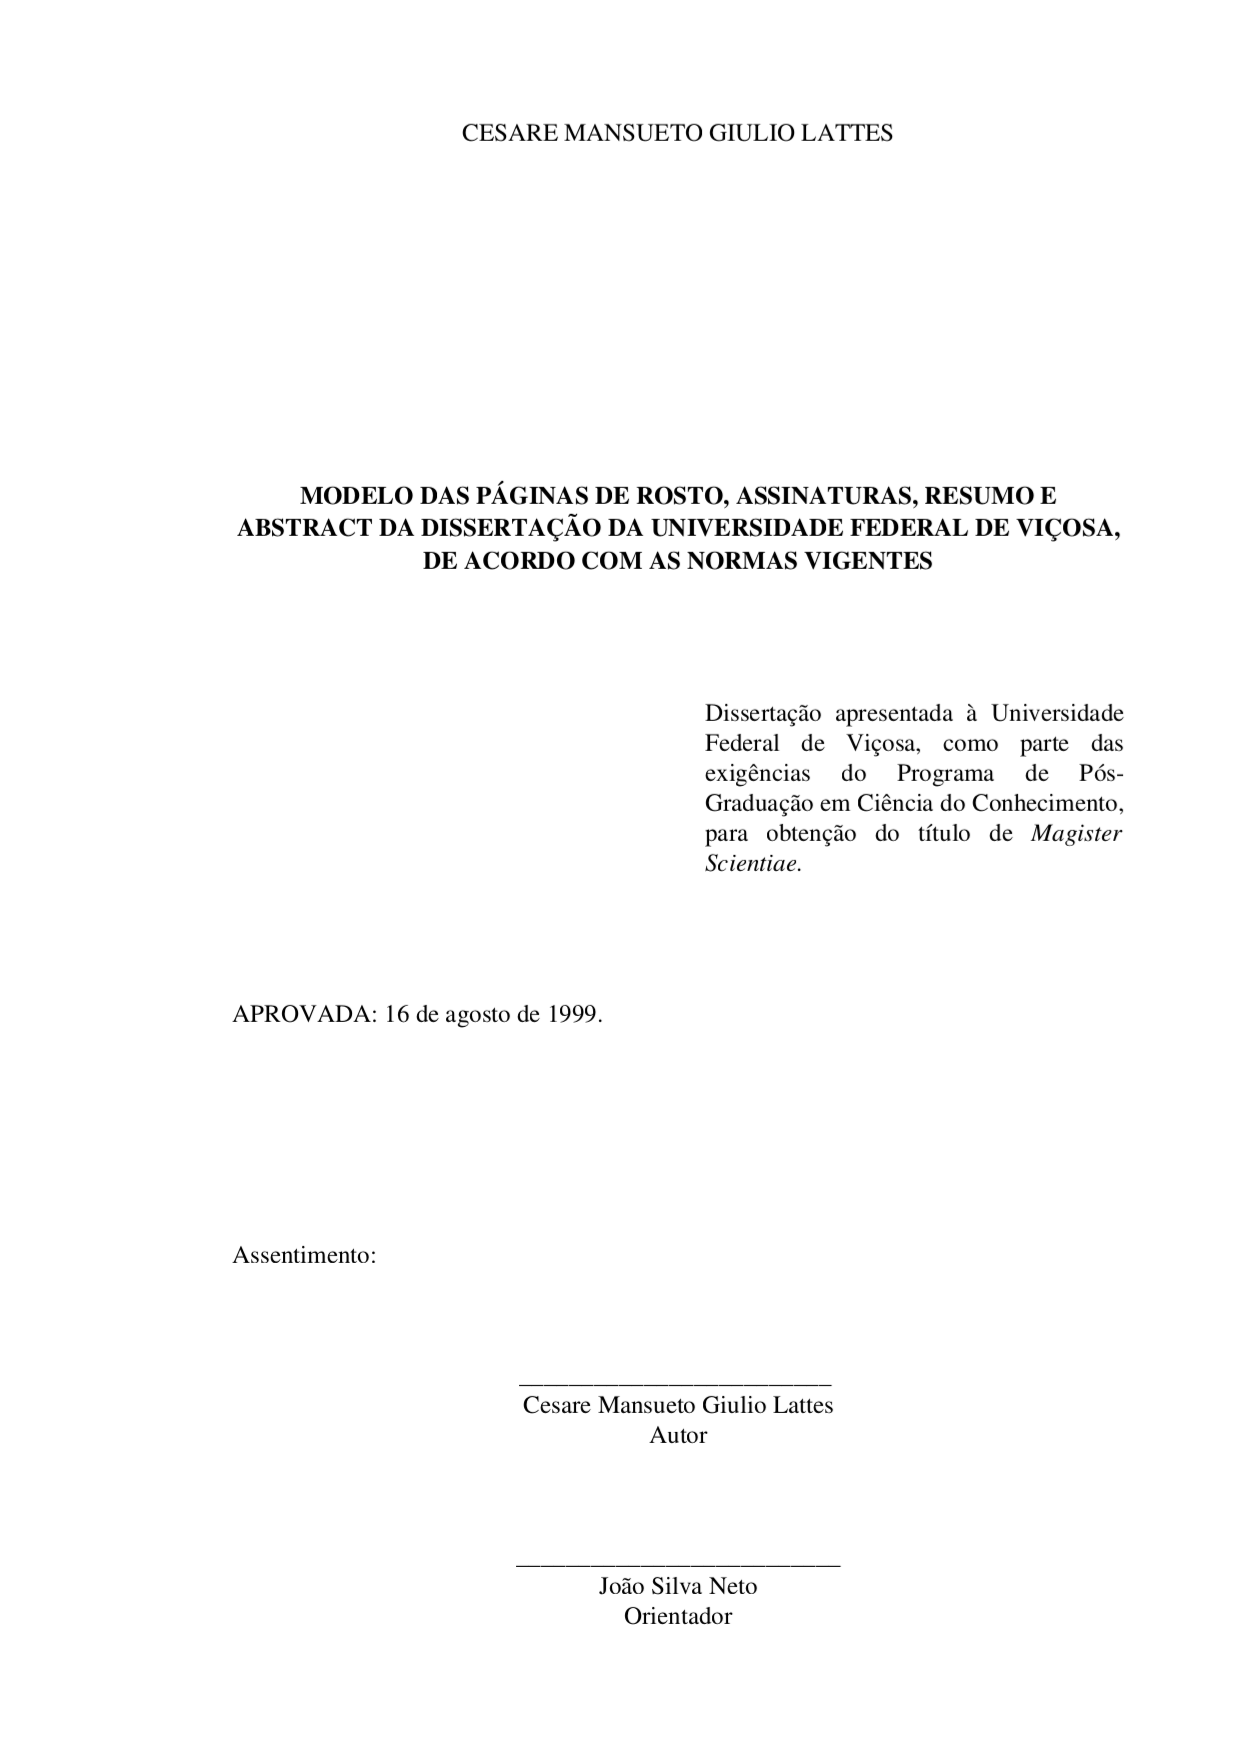
\includepdf[pages=-]{pdfs/Modelo-pgs-de-assinaturas.pdf}
%\imprimirfolhadeaprovacao

% Agradecimentos
\huge
\begin{center}
{\fontfamily{lmss}\selectfont Agradecimentos}
\end{center}
%\singlespacing
%\vspace{0.85cm}
\vspace{0.8cm}
\normalsize
AGRADECIMENTOS\\
O presente trabalho foi realizado com apoio da Coordenação de Aperfeiçoamento de Pessoal de Nível Superior – Brasil (CAPES) – Código de Financiamento 001.
\cleardoublepage

% RESUMOS

% resumo em português
\begin{resumo}[Resumo]
%\noindent

\vspace{0.35cm}
\singlespacing
DOE, John, M.Sc., Universidade Federal de Viçosa, junho de 2021. \textbf{Título da dissertação}. Orientador: Nome do orientador.

\vspace{\onelineskip}

%\onehalfspacing
\setstretch{1.5}
{
    RESUMO\\
}

\vspace{\onelineskip}

\noindent
\textbf{Palavras-chave}: Palavra-chave 1. Palavra-chave 2. Palavra-chave 3.

\end{resumo}

% resumo em inglês
\begin{resumo}[Abstract]
 \begin{otherlanguage*}{english}
   %\noindent
 
\vspace{0.35cm}
\singlespacing
DOE, John, M.Sc., Universidade Federal de Viçosa, June, 2021. \textbf{Título da dissertação em inglês}. Advisor: Nome do orientador.

\vspace{\onelineskip}

%\onehalfspacing
\setstretch{1.5}
{
    ABSTRACT\\
}

   \vspace{\onelineskip}

   \noindent
   \textbf{Keywords}: Keyword 1. Keyword 2. Keyword 3.
 \end{otherlanguage*}
\end{resumo}

% inserir lista de ilustrações
\pdfbookmark[0]{\listfigurename}{lof}
\listoffigures*
\cleardoublepage
% ---

% inserir lista de tabelas
\pdfbookmark[0]{\listtablename}{lot}
\listoftables*
\cleardoublepage

% ---
% Lista de siglas e abreviaturas (opcional)
% sintaxe: \item [sigla] Descrição da sigla

%\begin{siglas}
%\item[ABNT] Absurdas Normas Técnicas
%\item[UFV] Universidade Federal de Viçosa
%\end{siglas}

% Lista de símbolos (opcional)
% sintaxe: \item [simbolo] Descrição do símbolo

%\begin{simbolos}
%\item[$\infty$ ] Infinito
%\end{simbolos}

% inserir o sumario
\pdfbookmark[0]{\contentsname}{toc}
\tableofcontents*
\cleardoublepage
% ---

% ----------------------------------------------------------
% ELEMENTOS TEXTUAIS
% ----------------------------------------------------------
\textual

\chapter{Introdução}\label{cap:introducao}

Citação 1: \cite{mitchell1997learning}

\lipsum[2-4]

% ----------------------------------------------------------
% ELEMENTOS PÓS-TEXTUAIS
% ----------------------------------------------------------
\postextual

% Referências bibliográficas

\bibliography{references}

% Caso sejam necessários apêndices ou anexos em seu documento
% Use os ambientes abaixo

%% Apêndices
%
%% Inicia os apêndices
%\begin{apendicesenv}
%
%% Imprime uma página indicando o início dos apêndices
%\partapendices
%
%\chapter{Primeiro Apêndice}
%
%\chapter{Segundo Apêndice}
%
%\end{apendicesenv}
%
%
%% ----------------------------------------------------------
%% Anexos
%% ----------------------------------------------------------
%\begin{anexosenv}
%
%% Imprime uma página indicando o início dos anexos
%\partanexos
%
%\chapter{Primeiro Anexo}
%\lipsum[30]
%
%\chapter{Segundo Anexo}
%\lipsum[31]
%
%\end{anexosenv}

\end{document}
